\chapter{Реализация методов построения цифровых моделей рельефа и их сравнительный анализ}

\section{Подготовка исходных данных для построения матриц }

В данной работе описаны методы построения цифровых матриц, отражающих характеристики местности, таких как: матрицы залегания грунтовых вод, матрицы коэффициента фильтрации и матрицы коэффициента пористости, построенные по векторным картам, содержащим в себе по 13 исходных точек. В качестве исходных данных для построения векторных карт были использованы данные геодезической съемки, результаты исследования почвы в скважинах и в пределах продольных профилей рек. Для того, чтобы все матрицы получались одинаковыми по размеру, была создана рамка, как отдельная векторная карта (рисунок \ref{fig:9}).

\begin{figure}[h!]
    \center
    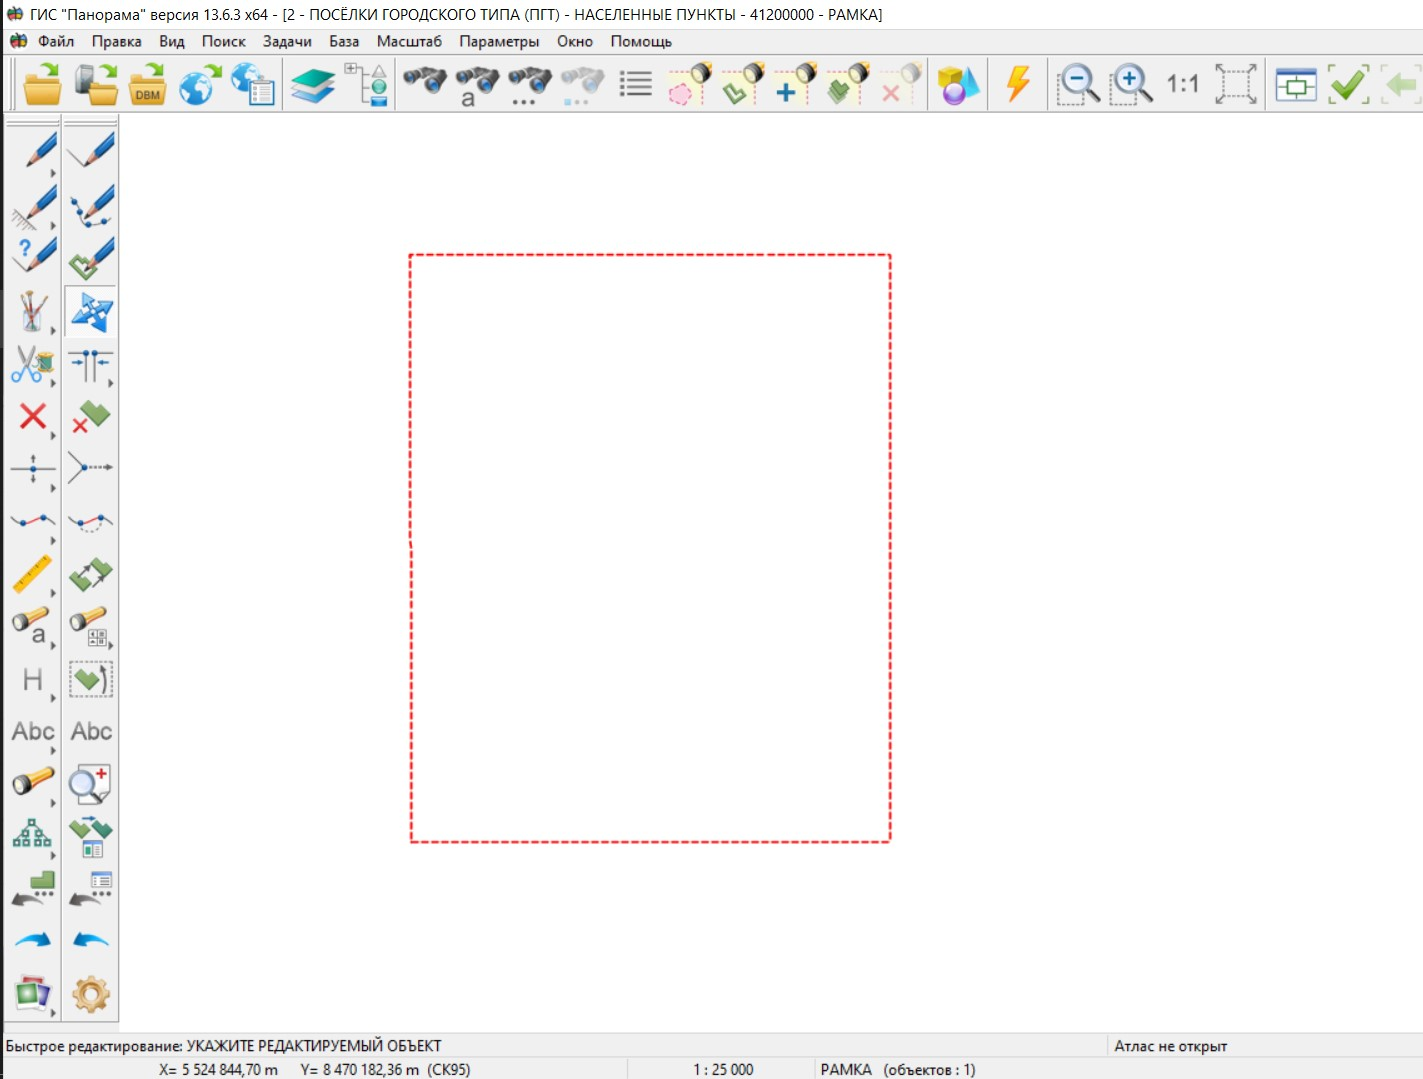
\includegraphics[scale=0.5]{images/1111.jpg}
    \caption{Векторная карта рамки}
    \label{fig:9}
\end{figure}


С помощью координат четырех точек были вычислены ширина и высота рамки, это необходимо для того, чтобы понять какую размерность будет иметь матрица на входе и выходе программы. Координаты были взяты из таблицы информации об объекте (рисунок \ref{fig:10}).

\begin{figure}[h!]
    \center
    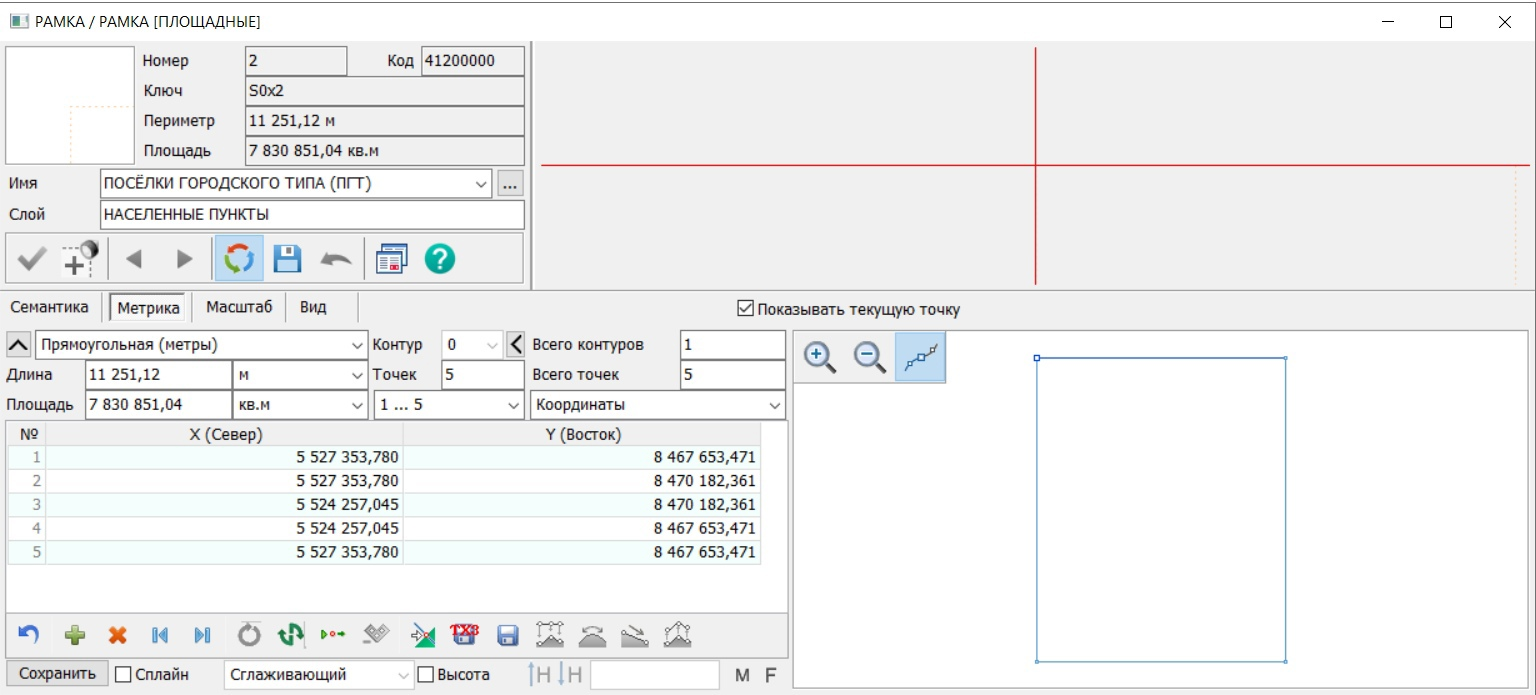
\includegraphics[scale=0.3]{images/222.jpg}
    \caption{Таблица с координатами рамки}
    \label{fig:10}
\end{figure}

Размер одного элемента в матрице равняется 15 метрам, исходя из этого делим ширину и высоту на размер одного элемента, для получения значений $N$ (количество столбцов матрицы) и $M$ (количество строк матрицы), полученная размерность: $N = 61$,  $M = 50$.

Так как для построения матриц качеств известно всего 13 значений, нужно достраивать матрицы определенного размера с помощью методов интерполяции, описанных ниже.

\section{Описание основных методов для построения цифровых моделей рельефа}

\subsection{Метод ReadFile для записи известных значений в матрицу из файла}

Метод ReadFile считывает и записывает в матрицу известные значения, которые расположены на векторной карте как точки (рисунок \ref{fig:11}). Те точки, которые нам неизвестны, заполнены нулями. Реализация метода ReadFile представлена в листинге \ref{ls:01}.

Для того, чтобы известные значения записывались в правильные ячейки матрицы, а именно, в тех же местах, что и на карте, необходимо из координат X и Y вычесть начальную координату X и Y рамки и поделить на размер элемента равный 15. Тогда все известные значения запишутся в те ячейки матрицы, в которых они находятся.

\begin{lstlisting}[caption={Метод ReadFile}, label={ls:01}]
static public void ReadFile(string file)
        {
            string line = "t";
            string[] splitLine;
            int X, Y;
            StreamReader sr = new StreamReader(file);

            while (line != null)
            {
                line = sr.ReadLine();
                try
                {
                    line = Regex.Replace(line," +", "");
                    line = Regex.Replace(line, "[.]", ","); 
                    splitLine = line.Split("|");
                    X = (int)((Double.Parse(splitLine[3])) - START_X) / H;
                    Y = (int)(Double.Parse(splitLine[4]) - START_Y) / H;
                    MATRIX[X, Y] = Double.Parse(splitLine[5]);
                    
                }
                catch { }
            }
        }
\end{lstlisting}

\begin{figure}[h!]
    \center
    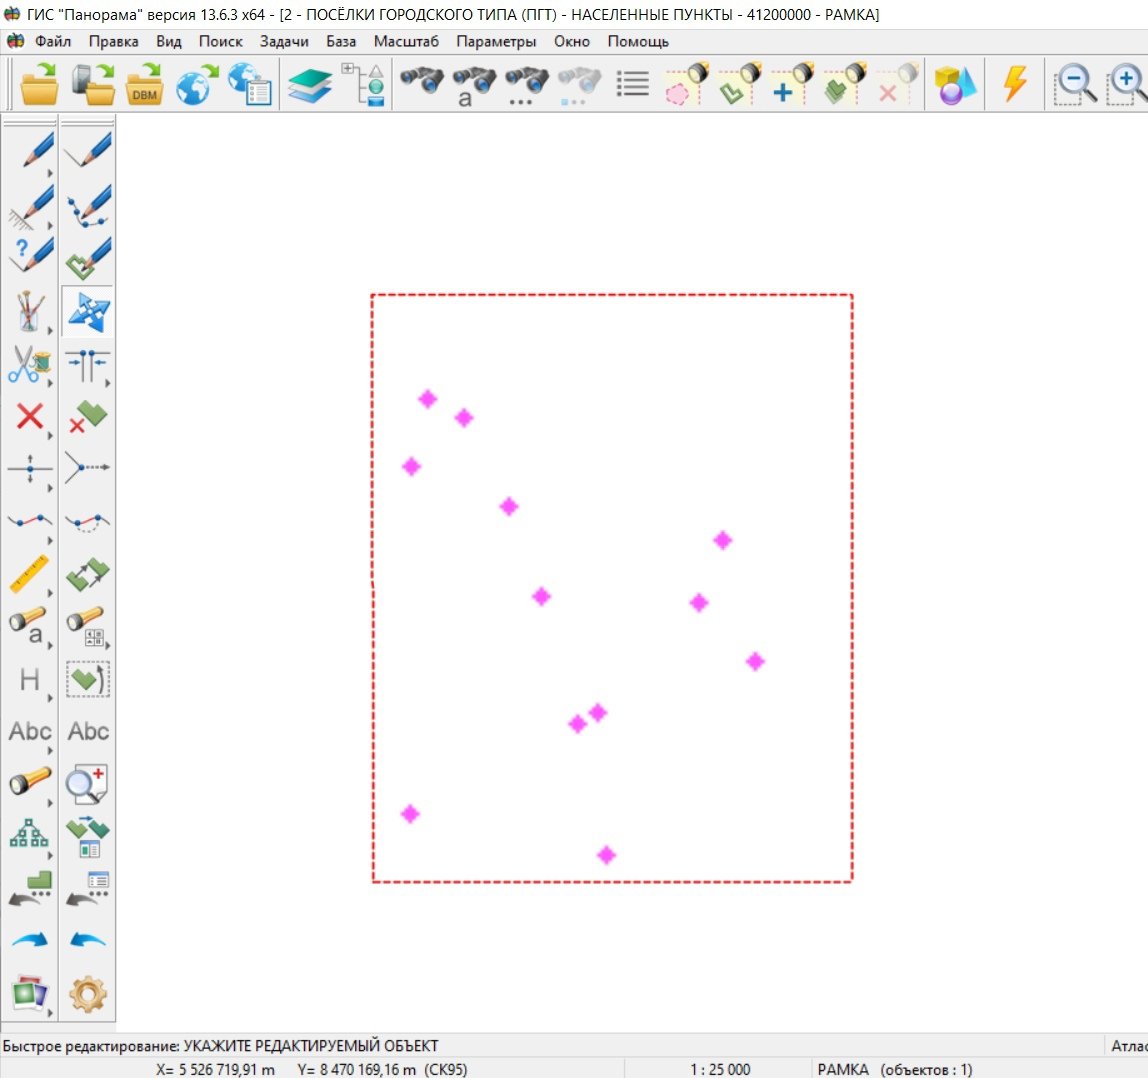
\includegraphics[scale=0.3]{images/333.jpg}
    \caption{Векторная карта с входными значениями}
    \label{fig:11}
\end{figure}


\subsection{Метод Calculate для заполнения неизвестных значений в матрице}

Данный метод заполняет значения матрицы, полученные с помощью метода интерполяции обратно взвешенных расстояний. Реализация данного метода представлена в листинге \ref{ls:02}.

\begin{lstlisting}[caption={Метод Calculate}, label={ls:02}]
        static double[,] calculate()
        {
            double[,] grid = new double[N,M];
            for(int i = 0; i < N; i++)
            {
                for(int j = 0; j < M; j++)
                {
                    grid[i,j] = idw(i, j);
                }
            }
            for (int i = 0; i < N; i++)
            {
                for (int j = 0; j < M; j++)
                {
                    if (MATRIX[i,j] != 0)
                    {
                        grid[i, j] = MATRIX[i, j];
                    }
                }
            }
            return grid;
        }
\end{lstlisting}

Полученную матрицу необходимо записать в файл, где в первом столбце содержится координата X, затем координата Y и значение в этой точке. Метод WriteFile представлен в листинге \ref{ls:03}. Выводится все в таком порядке не случайно, при импорте матрицы в ГИС Панораму необходимо указывать именно такой порядок значений. После отработки программы получаем выходной файл (рисунок \ref{fig:12}). 


\begin{lstlisting}[caption={Метод WriteFile}, label={ls:03}]
        static void writeFile(double[,] grid)
        {
            StreamWriter sw = new StreamWriter("filtr.txt");
            for (int i = 0; i < N; i++)
            {
                for (int j = 0; j < M; j++)
                {
                    sw.WriteLine(Convert.ToString(i * 50 + START_X) + " " + Convert.ToString(j * 50 + START_Y)+ " " + Convert.ToString(grid[i, j]));
                }
            }
        }
\end{lstlisting}

\begin{figure}[h!]
    \center
    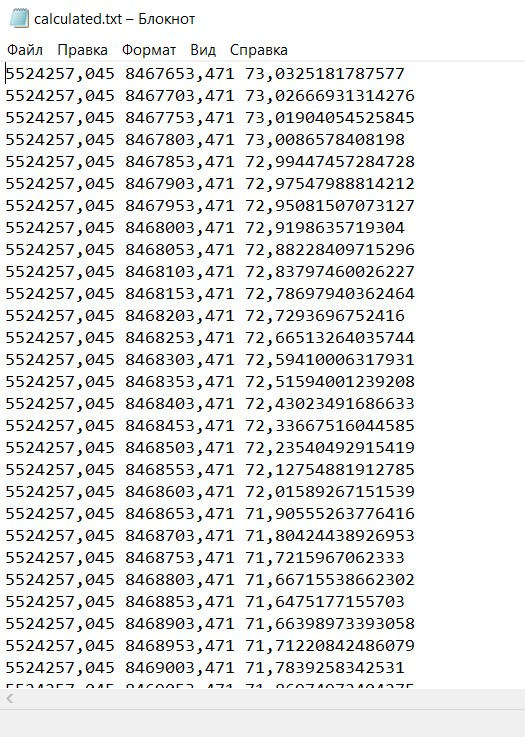
\includegraphics[scale=0.8]{images/555.jpg}
    \caption{Файл с выходными значениями}
    \label{fig:12}
\end{figure}

\subsection{Реализация метода интерполяции обратно взвешенных расстояний}

Для того, чтобы заполнить матрицу значениями, их необходимо посчитать. В листинге \ref{ls:04} приведена функция, которая реализовывает метод интерполяции обратно взвешенных расстояний, для нахождения значений в тех точках, что обозначены нулями по формуле \ref{e:f(p)}. 

\begin{equation} \label{e:f(p)}
f(\overline{p}) =  \frac{\sum_{i=1}^{n}{w_i(\overline{p}) * z_i}}{\sum_{i=1}^{n}{w_i(\overline{p})}},
\end{equation}
где \(w_i(\overline{p}) = \mid \overline{p}-\overline{p}_i \mid ^{-k}\) -- функция взвешивания обратного расстояния, $n$ -- количество опорных точек, $z_i$ -- значение функции в опорной точке, $\overline{p}$ -- координата искомой точки,  $\overline{p}_i$ -- координата опорной точки.

Для того, чтобы посчитать значение в точке $p$, необходимо рассчитать квадратный корень расстояния до известной точки и разделить значение $z$ в этой известной точке на посчитанный корень расстояния \cite{25, 27}. 

\begin{lstlisting}[caption={Метод средневзвешенной интерполяции}, label={ls:04}]
static double idw(int cx, int cy)
        {
            double res = 0, num = 0, denom = 0;
            for (int i = 0; i < 12; i++)
            {
                if(Math.Abs(Math.Pow(cx - _X[i], 2) + Math.Pow(cy - _Y[i], 2)) == 0)
                {
                    return 0;
                }
                else
                {
                    num += _Z[i] / Math.Abs(Math.Pow(cx - _X[i], 2) + Math.Pow(cy - _Y[i], 2));
                    denom += 1 / Math.Abs(Math.Pow(cx - _X[i], 2) + Math.Pow(cy - _Y[i], 2));
                }
            }
            res = num / denom;
            return res;
        }
\end{lstlisting}

\subsection{Реализация метода интерполяции сплайнами}

Сплайн интерполяция производится за счет создания поверхности, проходящей через все опорные точки при соблюдении условия минимальной кривизны \cite{24,26}. Сплайн-поверхность определяется формулой \ref{e:f(xy)}. 
\begin{equation} \label{e:f(xy)}
f(x,y) = \sum^N_{i=1} C_i *[(x - x_i)^2 + (y - y_i)^2] * ln[(x - x_i)^2 + (y- y_i)^2] + Ax + By + D,
\end{equation}
где $C_i$, $A$, $B$, $D$ -- некоторые постоянные коэффициенты, $(x_i, y_i)$ - координаты опорных точек.

Для нахождения коэффициентов, необходимо решить систему линейных алгебраических уравнений (СЛАУ) вида \ref{e:slau}. 

\begin{equation} \label{e:slau}
\begin{pmatrix}
 0 &  \phi_{12} & \phi_{13} & ... & \phi_{1n} & x_1 & y_1 & 1 \\ 
 \phi_{21} & 0 & \phi_{23} & ... & \phi_{2n} & x_2 & y_2 & 1 \\ 
 \phi_{31} & \phi_{32} & 0 & ... & \phi_{3n} & x_3 & y_3 & 1 \\ 
 ... & ... & ... & ... & ... & ... & ... & ... \\ 
 \phi_{n1} & \phi_{n2} & \phi_{n3} & ... & 0 & x_n & y_n & 1 \\ 
 1 & 1 & 1 & ... & 1 & 0 & 0 & 0 \\ 
 x_1 & x_2 & x_3 & ... & x_n & 0 & 0 & 0\\ 
 y_1 & y_2 & y_3 & ... & y_n & 0 & 0 & 0
\end{pmatrix} * \begin{pmatrix}
C_1\\ 
C_2\\ 
C_3\\ 
...\\ 
C_n\\ 
A\\ 
B\\ 
D
\end{pmatrix} = \begin{pmatrix}
z_1\\ 
z_2\\ 
z_3\\ 
...\\ 
z_n\\ 
0\\ 
0\\ 
0
\end{pmatrix},
\end{equation}
где $\phi_{ij}$ = $[(x_i - x_j)^2 + (y_i - y_j)^2] * ln[(x_i - x_j)^2 + (y_i - y_j)^2]$, $C_i$,A,B,D - искомые коэффициенты для сплайн-поверхности.

Для решения системы был выбран метод Гаусса для СЛАУ, так как неудалось привести матрицу к трехдиагональному виду для решения методом прогонки. В листинге \ref{ls:a:01} представлен метод реализующий подготовку матриц для решения СЛАУ методом Гаусса и заполнение интерполированных точек в сетку вывода.


\subsection{Реализация метода интерполяции с использованием радиально-базисной функции }
Радиально-базисной функцией называется функция зависящая от расстояния между искомой точкой и опорной точкой \cite{27}. В качестве радиально-базисной функции используется метрика Евклидового расстояния (формула \ref{e:Evk}). 
\begin{equation} \label{e:Evk}
\phi_i(x,y) = \sqrt{(x-x_i)^2 * (y-y_i)^2}.
\end{equation}

Функция интерполируется в данном методе с помощью взвешенной суммы радиально-базисных функций (формула \ref{e:sum}). 
\begin{equation} \label{e:sum}
f(x, y) = \sum ^N _{i=1} w_i*\phi_i(x,y) ,
\end{equation}
где $w_i$ -- веса.

Для того чтобы определить веса точек, необходимо решить систему уравнений \ref{e:sys2}. 
\begin{small}
\begin{equation} \label{e:sys2}
\begin{pmatrix}
1 & \phi_1(x_2, y_2) & \phi_1(x_3, y_3) & ... & \phi_1(x_n, y_n)\\ 
\phi_2(x_1, y_1) & 1 & \phi_2(x_3, y_3) & ... & \phi_2(x_n, y_n)\\ 
\phi_3(x_1, y_1) & \phi_3(x_2, y_2) & 1 & ... & \phi_3(x_n, y_n)\\ 
... & ... & ... & ... & ... \\ 
\phi_n(x_1, y_1) & \phi_n(x_2, y_2) & ... &  \phi_n(x_{n-1}, y_{n-1}) &  1\\ 
\end{pmatrix} * \begin{pmatrix}
w_1\\ 
w_2\\ 
w_3\\ 
...\\ 
w_n
\end{pmatrix} = \begin{pmatrix}
z_1\\ 
z_2\\ 
z_3\\ 
...\\ 
z_n
\end{pmatrix}
\end{equation}
\end{small}
Данная система решается методом Гаусса для СЛАУ. В листинге \ref{ls:a:02} представлен метод, реализующий подготовку матриц для решения СЛАУ методом Гаусса и заполнение интерполированных точек в сетку вывода.

\section{Сравнительный анализ результатов, полученных разными методами интерполяции}

В результате выполнения работы были построены матрицы залегания грунтовых вод, коэффициента пористости, коэффициента фильтрации тремя методами интерполяции, а именно методом интерполяции обратно взвешенных расстояний, методом интерполяции сплайнами и  методом интерполяции с использованием радиально-базисной функции. Данные матрицы были приведены к одному размеру в ГИС <<Панорама>>.

На рисунке \ref{fig:13} представлены матрицы а) залегания грунтовых вод, б) коэффициента пористости и в) коэффициента фильтрации, построенных с помощью метода обратно взвешенных расстояний.

\begin{figure}[h]
    \begin{minipage}[h]{0.3\linewidth}
    \center{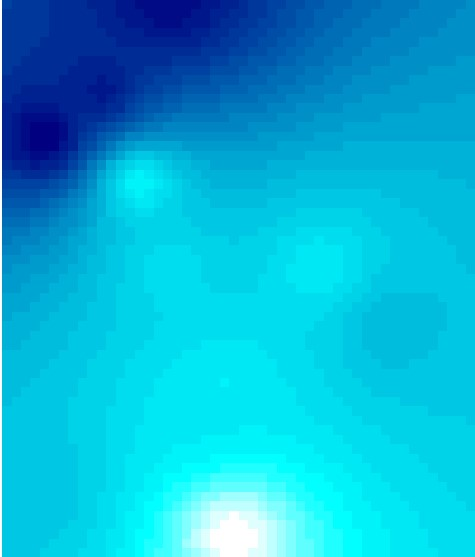
\includegraphics[width=1\linewidth]{images/mgobr.jpg} \\ а)}
    \end{minipage}
    \hfill
    \begin{minipage}[h]{0.3\linewidth}
    \center{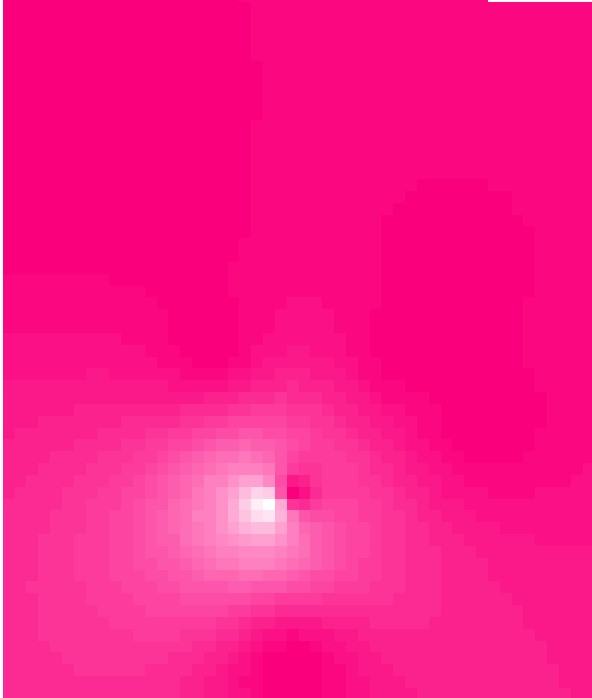
\includegraphics[width=1\linewidth]{images/mkpobr.jpg} \\ б)}
    \end{minipage}
    \hfill
    \begin{minipage}[h]{0.3\linewidth}
    \center{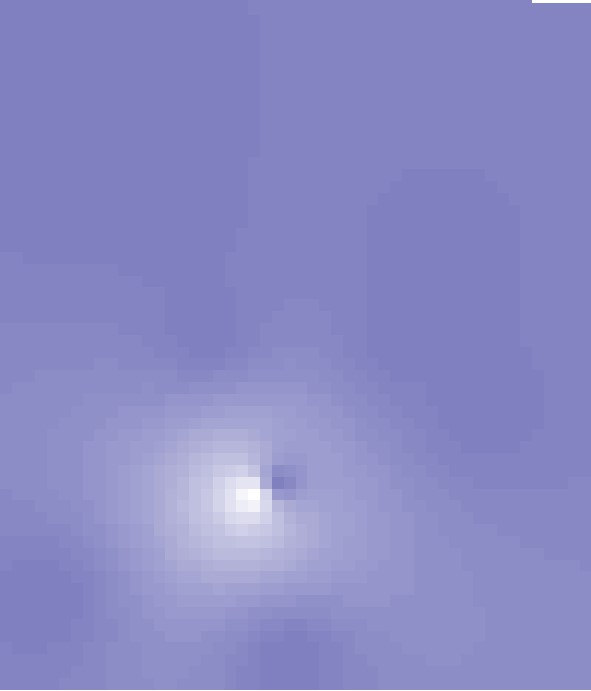
\includegraphics[width=1\linewidth]{images/mkfobr.jpg} \\ в)}
    \end{minipage}
\caption{Построенные матрицы методом обратно взвешенных расстояний}
\label{fig:13}
\end{figure}

На рисунке \ref{fig:14} представлены матрицы а) залегания грунтовых вод, б) коэффициента пористости и в) коэффициента фильтрации, построенных с помощью метода интерполяции сплайнами.

На рисункe \ref{fig:15} представлены матрицы а) залегания грунтовых вод, б) коэффициента пористости и в) коэффициента фильтрации, построенных с помощью метода с использованием радиально-базисной функции.

Можно заметить, что метод обратно взвешенных расстояний подходит для построения матриц с разрозненными исходными данными и их малым количеством, но при этом матрицы получаются не такими гладкими, как при построении методами интерполяции сплайнами и радиально-базисными функциями. Также метод построения сплайнами и радиально-базисными функциями плохо подходит для построения матриц с малым количеством исходных точек.

\begin{figure}[h]
    \begin{minipage}[h]{0.3\linewidth}
    \center{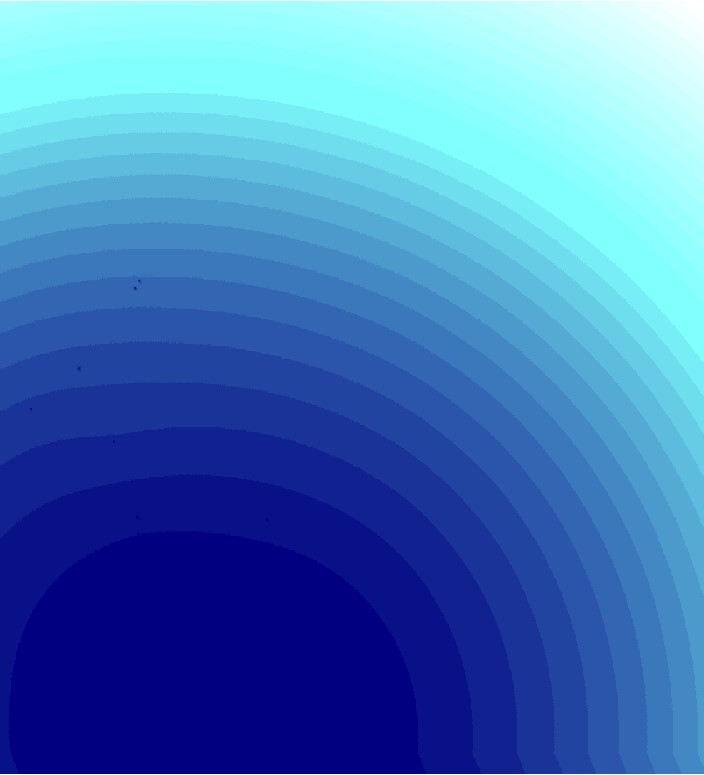
\includegraphics[width=1\linewidth]{images/mgs.jpg} \\ а)}
    \end{minipage}
    \hfill
    \begin{minipage}[h]{0.3\linewidth}
    \center{
\includegraphics[width=1\linewidth]{images/mkps.jpg} \\ б)}
    \end{minipage}
    \hfill
    \begin{minipage}[h]{0.3\linewidth}
    \center{
\includegraphics[width=1\linewidth]{images/mkfs.jpg} \\ в)}
    \end{minipage}
\caption{Построенные матрицы методом интерполяции сплайнами}
\label{fig:14}
\end{figure}

\begin{figure}[h]
    \begin{minipage}[h]{0.3\linewidth}
    \center{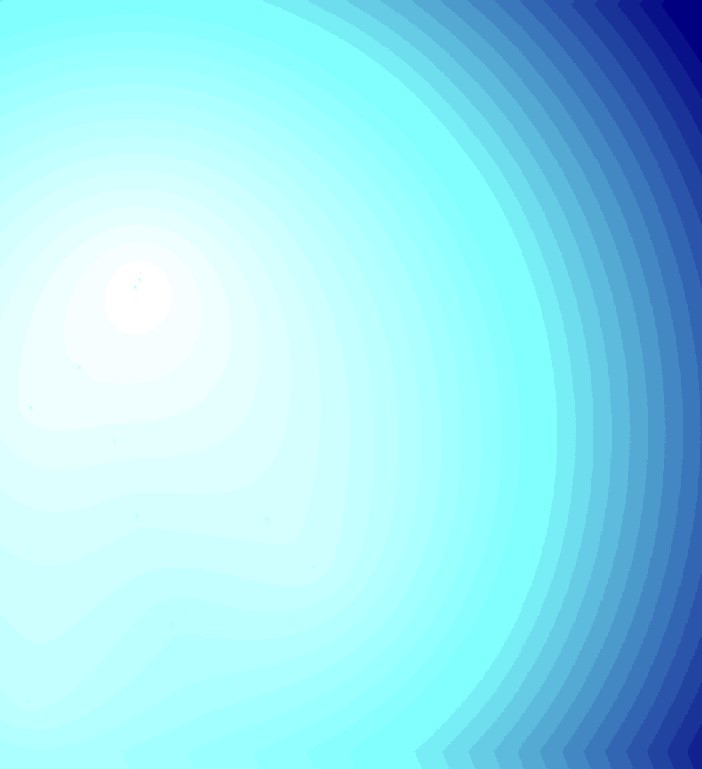
\includegraphics[width=1\linewidth]{images/mgrbf.jpg} \\ а)}
    \end{minipage}
    \hfill
    \begin{minipage}[h]{0.3\linewidth}
    \center{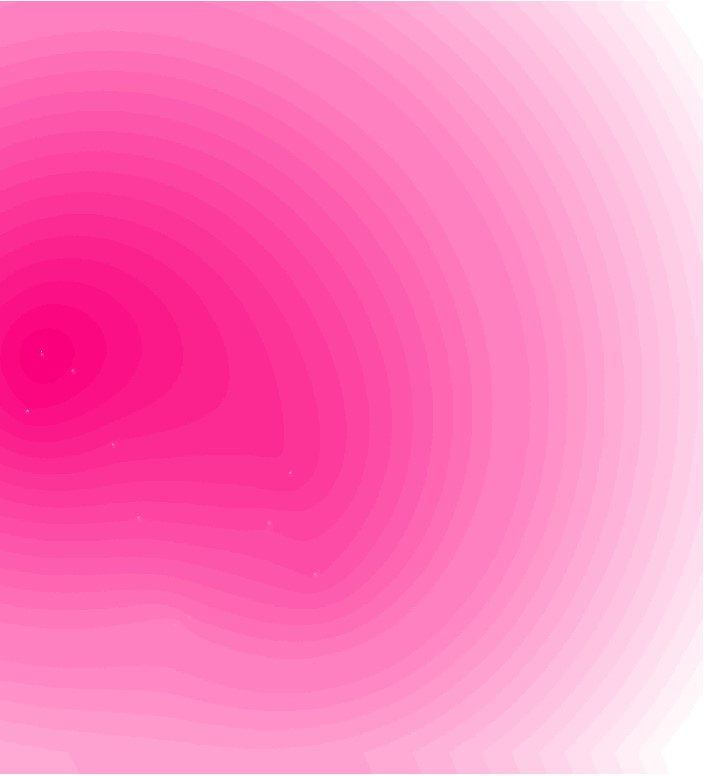
\includegraphics[width=1\linewidth]{images/mkprbf.jpg} \\ б)}
    \end{minipage}
    \hfill
    \begin{minipage}[h]{0.3\linewidth}
    \center{
\includegraphics[width=1\linewidth]{images/mkfrbf.jpg} \\ в)}
    \end{minipage}
\caption{Построенные матрицы методом c использованием метода радиально-базисной функции}
\label{fig:15}
\end{figure}

